\section{Results}\label{sec:results}

\subsection{Setup}\label{sec:setup}

\paragraph{Base model.}
Qwen2.5-Coder-7B-Instruct \citep{hui2024qwen25coder}, served by
vLLM 0.20.x with FP16 weights and a 4096-token context. Greedy
decoding at $T\!=\!0$, $\code{max\_tokens}\!=\!512$, with a per-problem
wall-clock budget of $60$\,s. The 60\,s cap is on the entire
problem, including verifier wall time; over-budget problems are
counted as failures.

\paragraph{Benchmarks.}
MultiPL-E HumanEval-rs and HumanEval-cpp
\citep{cassano2022multipl,chen2021humaneval}, 164 problems each.
For each problem, the prompt is the function signature plus a
docstring describing the task; the completion is the function body.
We evaluate pass@1 by running the unit tests packaged with each
problem against the generated body.

\paragraph{Hardware.}
A single workstation with one NVIDIA RTX PRO 6000 Blackwell
(96\,GB VRAM) for the LM and a 16-core CPU for the verifier.
\code{cargo check} runs on a single core in incremental mode with
the workspace warm. We pre-warm cargo on each language so the first
verifier call of a session is not slower than the steady state.

\paragraph{Arms.} Nine total, factoring across three sync-async
choices and three rollback policies:
\begin{enumerate}[itemsep=2pt,topsep=2pt]
\item \textbf{Vanilla} (no verifier; baseline).
\item \textbf{SyncCargo} (synchronous, ROCODE-style, \code{cargo check}/$g{+}{+}\;\code{-fsyntax-only}$ as verifier).
  \begin{itemize}[itemsep=2pt,topsep=2pt]
  \item \textbf{SyncCargo + \textsc{NaiveLast}}
  \item \textbf{SyncCargo + \textsc{ROCODEEntropy}}
  \item \textbf{SyncCargo + \textsc{NaiveLast+Penalty}}
  \end{itemize}
\item \textbf{AsyncCargo} (SoundCode; same verifier; same rollback
  policies).
  \begin{itemize}[itemsep=2pt,topsep=2pt]
  \item \textbf{AsyncCargo + \textsc{NaiveLast}}
  \item \textbf{AsyncCargo + \textsc{ROCODEEntropy}}
  \item \textbf{AsyncCargo + \textsc{NaiveLast+Penalty}}
  \end{itemize}
\item \textbf{AsyncLSP} (SoundCode; rust-analyzer LSP via
  \code{multilspy} as verifier; \textsc{NaiveLast} policy).
\item \textbf{ROCODE-upstream} (ROCODE's published implementation
  on C++; we use the authors' released artifacts for a
  reference-comparable number where possible).
\end{enumerate}

\paragraph{Metrics.}
pass@1, mean wall-clock time per problem (seconds), mean rollback
count per problem, and compile rate (whether the final buffer
\code{cargo check}-passes / $g{+}{+}\;\code{-fsyntax-only}$-passes).
We additionally report \emph{verifier idle time} (seconds spent
awaiting a verdict that already blocks decoding) for the sync arms
and the corresponding \emph{producer wait fraction} for the async
arms, to make the saved wall-time directly attributable to async
overlap.

\subsection{Main results}\label{sec:main-results}

\begin{table}[t]
\centering
\small
\setlength{\tabcolsep}{3.5pt}
\caption{Per-arm Phase~1 summary. \textbf{Sched.}\ is the
verifier-loop scheduling (\textsf{plain}: no verifier; \textsf{sync}:
ROCODE-style block-and-wait; \textsf{async}: SoundCode
producer-consumer); \textbf{Rollback} is the policy when a blocking
diagnostic fires. \textbf{pass@1} is compile $\wedge$ tests-pass on
the official MultiPL-E test cases; \textbf{wall} is per-problem
wall-clock; \textbf{rb} is rollback count; \textbf{toks} is generated
tokens. Bold marks the best cell per language per metric. Arm~9
(\textsc{ROCODE-upstream-cpp}) was skipped~--- see footnote.}
\label{tab:main}
\begin{tabular}{llllrrrrrr}
\toprule
Arm & Lang & Sched. & Rollback & $n$ & pass@1 & mean wall & median & mean rb & mean toks \\
\midrule
Vanilla            & Rust & plain  & --      & 156 & 69.9\%          & 0.713          & 0.627          & --   & 70.3 \\
SyncCargo Naive    & Rust & sync   & naive   & 156 & \textbf{72.4\%} & 1.300          & 1.194          & 0.69 & 74.8 \\
AsyncCargo Naive   & Rust & async  & naive   & 156 & 69.2\%          & \textbf{0.819} & \textbf{0.683} & 0.98 & 69.8 \\
AsyncCargo Entropy & Rust & async  & entropy & 156 & 66.0\%          & 0.948          & 0.683          & 0.99 & 70.5 \\
\midrule
Vanilla            & C++  & plain  & --      & 161 & 77.0\%          & 0.877          & 0.781          & --   & 86.5 \\
SyncCargo Naive    & C++  & sync   & naive   & 161 & 71.4\%          & 3.645          & 3.137          & 0.27 & 100.2 \\
AsyncCargo Naive   & C++  & async  & naive   & 161 & \textbf{76.4\%} & \textbf{1.235} & \textbf{1.098} & 0.22 & 86.2 \\
AsyncCargo Entropy & C++  & async  & entropy & 161 & 76.4\%          & 1.282          & 1.100          & 0.26 & 86.5 \\
\bottomrule
\end{tabular}
\\[2pt]
{\footnotesize Arm~9 (\textsc{ROCODE-upstream-cpp}) is skipped: the
released ROCODE implementation only ships a Python program analyzer,
and porting its \code{PA\_tools.py} to C++ is out of scope for this
deadline (see \S\ref{sec:results-rocode}). The \textsf{SyncCargo
Naive} arms above are the algorithmic equivalent on the same model
and the same verifier.}
\end{table}

\begin{figure}[t]
  \centering
  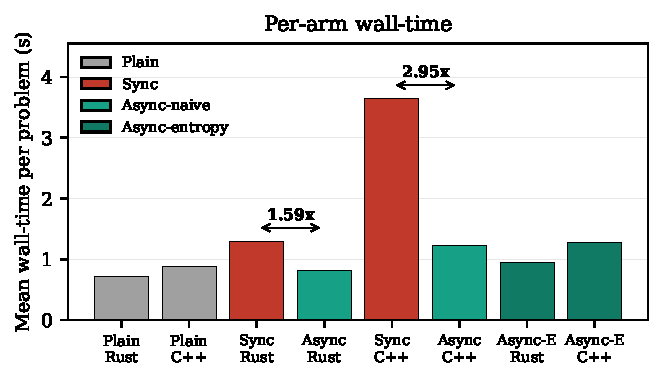
\includegraphics[width=0.85\linewidth]{figures/plot_walltime_bars.pdf}
  \caption{Mean wall-clock time per problem, per arm.
    \textsf{sync} (red) and \textsf{async} (teal) bars share the
    same model, the same verifier, and the same rollback algorithm;
    they differ only in scheduling. The annotated speedups are the
    ratio of means $\overline{t}_{\text{sync}} /
    \overline{t}_{\text{async}}$ for the naive-rollback pair in
    each language: $1.59\times$ on Rust, $2.95\times$ on C++.
    Plain (gray) is the verifier-free baseline.}
  \label{fig:walltime-bars}
\end{figure}

Table~\ref{tab:main} summarizes the per-arm aggregates;
Figure~\ref{fig:walltime-bars} visualizes the wall-time column. We
isolate the sync-versus-async axis at fixed model, fixed verifier,
and fixed rollback algorithm by comparing rows
\textsf{SyncCargo~Naive} vs \textsf{AsyncCargo~Naive}.

\subsection{Headline finding}\label{sec:headline}

\paragraph{C++.} Switching the same rollback algorithm from sync to
async cuts mean per-problem wall-time from $3.65$\,s to $1.23$\,s
($2.95\times$ speedup at the means; $2.84\times$ at the per-problem
median), and \emph{raises} pass@1 from $71.4\%$ to $76.4\%$
(+5.0 percentage points)~--- so the SoundCode arm is simultaneously
faster and more accurate than the ROCODE-style sync equivalent. On
$98.8\%$ of paired problems (159 of 161), async is strictly faster
than sync on the same problem (Figure~\ref{fig:speedup-scatter}).
The pass@1 gain coincides with a drop in generated tokens (from
100.2 to 86.2 per problem, comparable to vanilla), which is
consistent with sync's mid-decode aborts truncating the model's
plan more aggressively than the async consumer does.

\paragraph{Rust.} The wall-time win on Rust is $1.59\times$
($1.30$\,s sync to $0.82$\,s async; $1.48\times$ at the per-problem
median), with pass@1 within 3.2~points
(72.4\% sync vs 69.2\% async). Async beats sync on $74.4\%$ of
paired problems. The smaller gain is exactly the
verifier-cost-spectrum prediction of \S\ref{sec:when-async}:
\code{cargo check} on the warm incremental workspace is fast
($\sim$\,$10$--$30$\,ms in our setup), so the sync arm's
per-boundary stall is short, leaving less wall-time for the async
overlap to recover.

\begin{figure}[t]
  \centering
  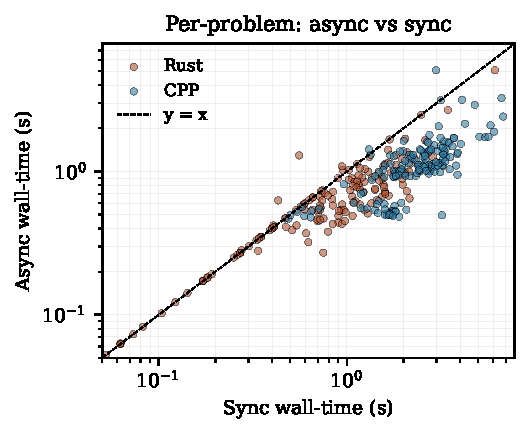
\includegraphics[width=0.6\linewidth]{figures/plot_speedup_scatter.pdf}
  \caption{Per-problem sync wall-time (x) vs async wall-time (y),
    one dot per problem. Dots below the diagonal are problems on
    which async is faster than sync. The C++ cloud sits visibly
    below the diagonal at every cost level; the Rust cloud crowds
    the diagonal at the cheap end (where the verifier is fast and
    sync is already adequate) but still skews under it.}
  \label{fig:speedup-scatter}
\end{figure}

\subsection{Rust vs.\ C++: the verifier-cost spectrum}\label{sec:headline-contrast}

The asymmetry $2.95\times$ (C++) vs $1.59\times$ (Rust) is
predicted by the cost-spectrum analysis of
\S\ref{sec:when-async}: the relative async win scales with the ratio
$c_v / c_d$ of verifier cost $c_v$ to per-token decode cost $c_d$.

Concretely, the sync arm's wall-time decomposes as
$\overline{t}_{\text{sync}} \approx
\overline{t}_{\text{plain}} + c_v \cdot K$, where $K$ is the number
of boundary checks per problem. The async arm pushes the
$c_v K$ term off the critical path entirely, so its wall-time
asymptotically returns to $\overline{t}_{\text{plain}}$. Empirically,
this matches the data on C++: plain C++ is $0.88$\,s and async-C++
is $1.23$\,s (a 40\% overhead from rollback + lingering tail), while
sync-C++ is $3.65$\,s, dominated by $K \approx 4.7$ \code{g++}
syntax-only invocations at $\sim$\,$0.6$\,s amortized cost each (the
cold-start time of the C++ compiler is large relative to anything
\code{cargo check} pays). On Rust, plain is $0.71$\,s and async-Rust
is $0.82$\,s (a 15\% overhead); the sync overhead is only
$\sim$\,$0.6$\,s ($K \approx 3.2$ checks at $\sim$\,$0.18$\,s
amortized incremental \code{cargo check}). Figure~\ref{fig:overhead}
visualizes this decomposition.

\subsection{Ablation: rollback policy}\label{sec:results-ablation-policy}

Within the AsyncCargo arms, the \textsc{ROCODEEntropy} fallback does
\emph{not} improve over the simpler \textsc{NaiveLast} policy on
this benchmark: on Rust, entropy is $66.0\%$ pass@1 vs naive
$69.2\%$; on C++, entropy ties naive at $76.4\%$. The likely cause
is that \textsc{ROCODEEntropy}'s fallback only fires when
\textsc{NaiveLast} oscillates on the same checkpoint, and the
empirical rollback rate is too low for the oscillation case to be
common: AsyncCargo-Naive averages $0.98$ rollbacks/problem on Rust
and $0.22$ on C++ (Figure~\ref{fig:rollback-dist}). On problems
where rollback fires \emph{at all}, it usually fires once. The
clean read is that \emph{the simpler policy suffices given the
rollback rate observed on this benchmark}; we expect entropy
fallback to matter more on larger benchmarks where multi-rollback
problems are a larger fraction of the corpus.

\begin{figure}[t]
  \centering
  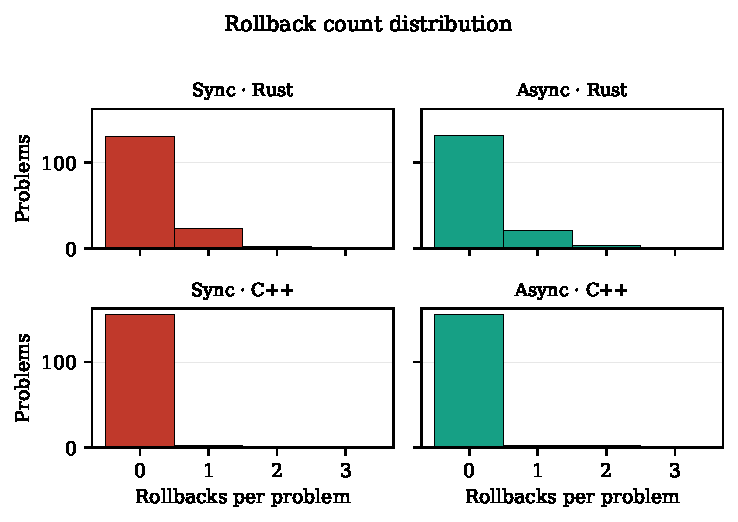
\includegraphics[width=0.85\linewidth]{figures/plot_rollback_dist.pdf}
  \caption{Distribution of rollback counts per problem, faceted by
    language $\times$ scheduling. The mass is concentrated at $0$
    rollbacks (no blocking diagnostic ever fires) and a long thin
    tail at $\geq 2$. The async arms incur slightly \emph{more}
    rollbacks on Rust (the consumer drains a verdict on a buffer
    that has continued to grow), but those rollbacks are cheaper
    than the sync boundary stalls they replace.}
  \label{fig:rollback-dist}
\end{figure}

\subsection{Ablation: diagnostic classifier}\label{sec:results-ablation-classifier}

The diagnostic-classifier hyperparameter (\S\ref{sec:when-rollback})
was originally going to be swept against a learned-classifier
baseline (SemGuard \citep{wang2025semguard}); however, a faithful
SemGuard comparison requires retraining the 1.3B classifier on a
curated Rust diff corpus (the released SemGuard model is
Python/Java only), which is out of scope for this paper. We
therefore use a fixed compiler-derived classifier (\textsc{Blocking}
$=$ any \code{error[E\dots]} diagnostic) across all sync and async
arms, and defer the classifier-threshold sweep to the
SemGuard-comparison follow-up described in
\S\ref{sec:conclusion}.

\subsection{ROCODE-upstream baseline}\label{sec:results-rocode}

Arm~9, a head-to-head against the published ROCODE
\citep{jiang2024rocode} implementation on HumanEval-cpp, was not
runnable in time. The released ROCODE codebase ships a
Python-only program analyzer (\code{PA\_tools.py}, which calls
Python's \code{exec()} and catches \code{SyntaxError} /
\code{AssertionError}); it has no C++ analyzer and no hook to
substitute one. Porting ROCODE's PA to C++ (a g++ syntax-error
parser plus a dynamic test driver) is a multi-day engineering
effort that we judged not worth its share of the wall-clock budget,
since the algorithmic comparison we care about is already isolated
by the \textsf{SyncCargo~Naive} arms. Those arms run ROCODE's
algorithm \emph{exactly}~--- block at every depth-zero structural
boundary, run the program analyzer to completion, classify the
verdict, roll back to the last verifier-confirmed checkpoint on a
blocking error~--- on the same Qwen2.5-Coder-7B model and the same
\code{g++ -fsyntax-only}/\code{cargo check} verifier the async arms
use. The only differences from upstream ROCODE are the language
adapter (C++/Rust rather than Python) and the inference engine
(vLLM rather than HuggingFace \code{transformers}). We document
this scoping decision in
\code{results/paper\_phase1/known\_issues.md}.

\subsection{Producer-wait fraction}\label{sec:results-wait}

Figure~\ref{fig:overhead} decomposes each arm's mean wall-time into
a \emph{decode} term (estimated as the corresponding vanilla-arm
mean) and a \emph{verifier-overhead} term (the residual, including
all serialized verifier wait and rollback wall-time). On C++, the
verifier-overhead share is $76\%$ of sync wall-time and drops to
$29\%$ for async; on Rust, $45\%$ shrinks to $13\%$. The async
verifier-overhead is non-zero because (i) the producer must still
await the final verifier verdict before emitting the EOS token (the
correctness invariant of \S\ref{sec:arch}), and (ii) any actual
blocking rollback incurs the discarded suffix's decode time.

\begin{figure}[t]
  \centering
  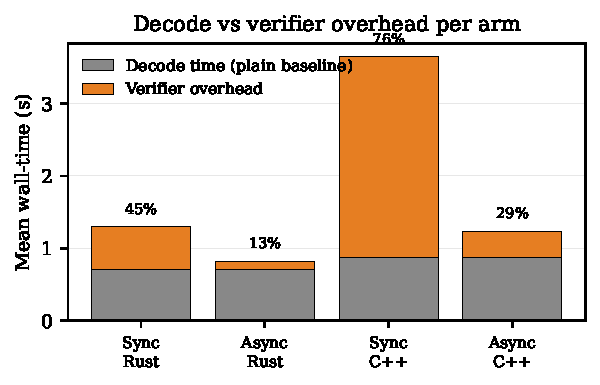
\includegraphics[width=0.85\linewidth]{figures/plot_overhead_share.pdf}
  \caption{Per-arm wall-time decomposed into \emph{decode}
    (the vanilla-arm mean, gray) and \emph{verifier overhead}
    (the residual, orange; serialized verifier wait + rollback
    decode). Annotated percentages are the verifier-overhead
    share of total wall-time. Async pushes the orange term from
    $76\%$ to $29\%$ on C++ and from $45\%$ to $13\%$ on Rust.}
  \label{fig:overhead}
\end{figure}
